\documentclass[a4paper,sans]{article}
\usepackage[left=2.5cm,right=2.5cm]{geometry}
\usepackage[UTF8]{ctex}
\usepackage{graphicx}
\usepackage{amsmath}
\usepackage{subfigure} %绘制子图包
\def\figureautorefname{Fig}
\renewcommand{\figurename}{Fig}
\usepackage[colorlinks,
linkcolor=blue,
anchorcolor=red,
citecolor=green
]{hyperref}
\bibliographystyle{naturemag}
\linespread{1.5}
\begin{document}
\begin{flushleft}
English Name : Frank\\
Chinese Name : 樊云谊\\
Student ID : 202018001436031
\end{flushleft}
\begin{center}
	\zihao{3}
	\textbf{The Usage of SAXS Method in Polymer Area}
\end{center}
	\zihao{5}
	\section{Introduction} % (fold)
	\label{intro}
	Small Angle X-ray Scattering (SAXS for short) is an experimental method widely used in material characterization, such as polymers, metals and solution systems. The incident wave passes its own energy to the electrons. The electrons transform the energy by scattering X-ray which has the same frequency as the incident wave. This phenomenon is called \textit{\textbf{scattering}}. \cite{RN102} The scatter angle is the angle between incident direction and reflection direction, always noted as $2\theta$. When $2\theta < 5^{o}$, it is called small angle scattering; when $2\theta > 5^{o}$, it is called wide angle scattering.\cite{RN59}
	

	In polymer research area, the crystallization condition is a key issue. Because it  deeply influences the physical properties, such as dynamic properties, thermo properties and optical properties. \cite{RN40}Using the SAXS detection method, X-ray intensity data was collected and used to calculate lots of information, including the long period, the radius of gyration and crystallinity. For some microstructures, a polarized optical microscope(POM) was used to locate the research position of polymer material. Consequently the SAXS method was used. SAXS and POM were used to study the dynamic property of blend materials of PCL and PLA.\cite{RN35}


	The hypothesis of the research is that the stretching direction of the PLA fibers has a great effect on the formation of PCL crystalls. To test this hypothesis, the following experiment was carried.

\newpage
	\section{Method and Results} % (fold)
	\label{sec:method}
	% subsection experiment (end)
	First of all, compoud reflective lens (CRLs) were used to minilize the X-ray pattern to a micron level. For the characterization of polymer material, X-ray energy at 7-15keV is required. Berylium quality CRLs were chosen to ensure a minimum flux at $10^{10}$ photons/s. \cite{RN43}


	For the next stage, the spatial attitude of POM was adjusted with a step motor, aimed changing 5 spatial directions. X-ray coild passed the CRLs through this method. Once the flux was enough, scintillation crystal CsI was set up to locate the coordinator of X-ray pattern on a CCD camera. Then the samples were put on the experimental platform,taking pictures by POM and collecting data with a synchrotron detector.\cite{RN42}


	Meanwhile, the preparation of the sample was carried. The sample was the blend of Poly-caprolactone (PCL) and Poly-lactide(PLA). Then electrospin method was used to make the blend's membrane with different mass ratio. Using tensile device to enlongate the membrane. The membrane was put into a 80 $^{o}C$ environment and stayed for 3 hours After that it was transfered into a 30$^{o}C$ environment and stayed for 30 minutes to make the content crystallize.\cite{RN38}


	Eventually, certain physical properties was measured using the SAXS method.
	A SAXS device(beamline BL19U2, Shanghai Synchrotron Radiation Facility, SSRF, Shanghai, China) was used to study the crystal lamellar structure of the samples at room temperature.
	 A Pilatus 1M detector(981 $\times$ 1043 pixels with a pixel size of 172 $\mu$m) was performed to collect SAXS patterns. 
	The X-ray wavelength was 0.1033 nm, and the sample to decector distance was set at 2700mm.
	 Structure information data of the crstall region and the amorphous region were collected respectively. 
	 The dynamic tensile data was also collected. 
	 DSC data was measured to get the thermo property.\cite{RN102} A METTlER DSC was used to obtain the relationship between heat flow and temperature.
	
	% subsection result (end)
	
	% section discussion_and_conclusion (end)
	% section m (end)
	\section{Discussion and Conclusion} % (fold)
	\label{sec:discussion_and_conclusion}
		The aim of this study was to determine the phase morphology and the crystallization behavior of the PCL/PLA polymer blends.
		By adjusting the enlongation rates of the electrospun membrane, blends with different enlongation rate were obtained. 
		As the enlongation rate increased, the orientation of fibers inside the blends were grdually unified into one direction. Consequently, the dynamic properties obviously changed . 


		As shown in \autoref{fig:POM}, the PLA fibers stretch along the same direction gradually as the enlongation rate increases. This phenomenon induces the crystallization of PCL,presenting orientation as shown in \autoref{fig:SAXS}.
	\begin{figure}[ht]
		\centering
		\subfigure[POM result of PLA/PCL blend]{
		\label{fig:POM}
		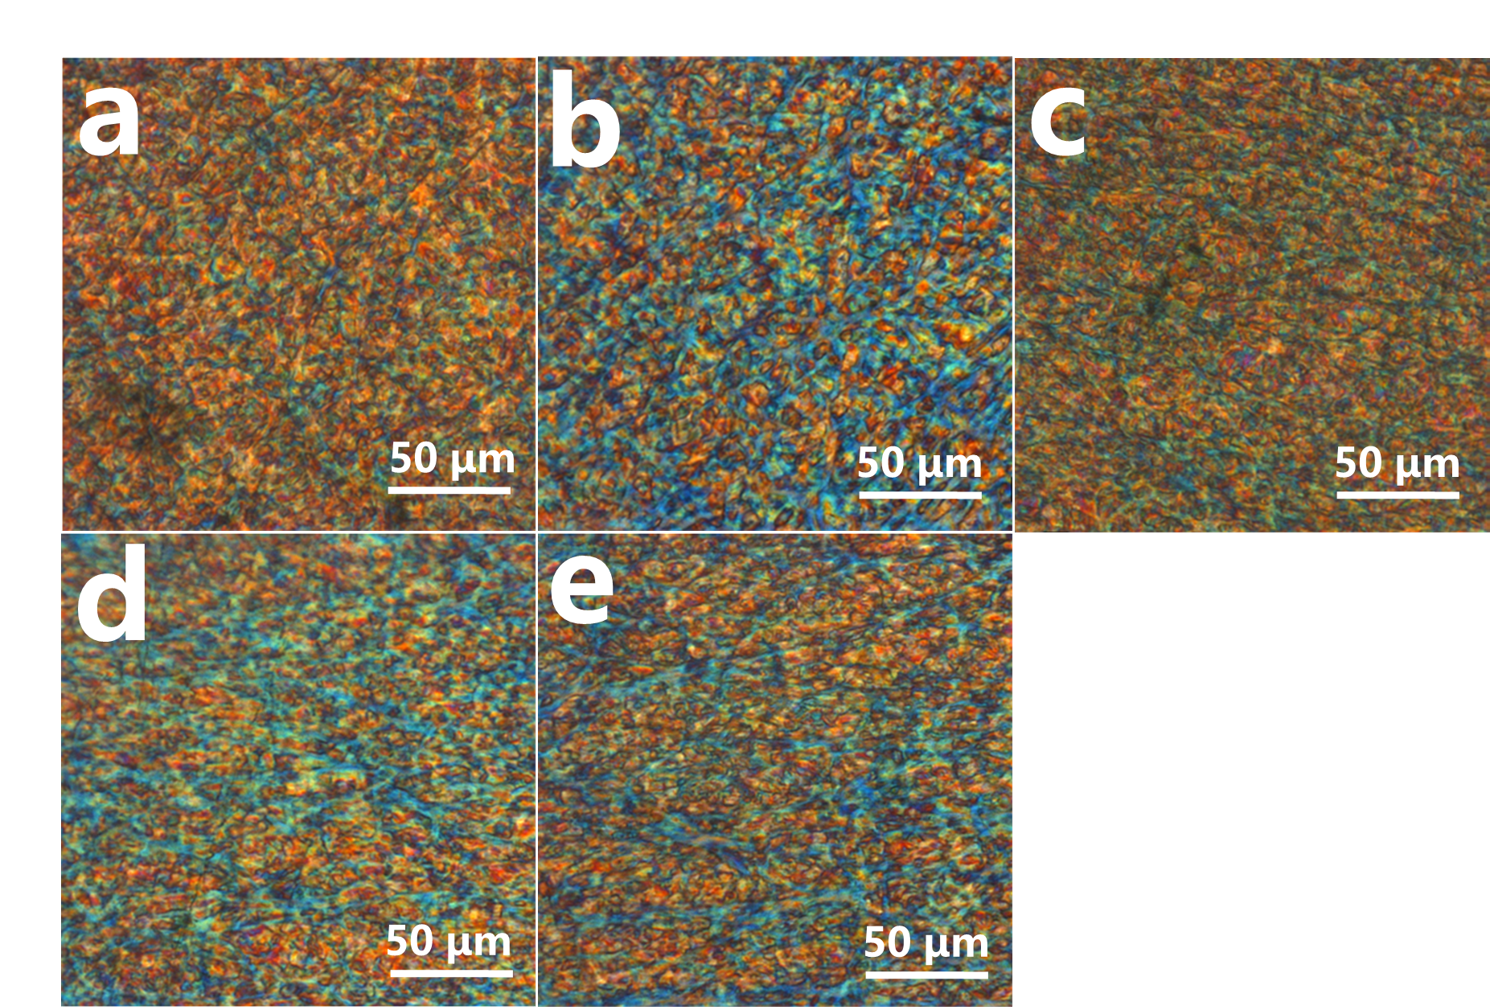
\includegraphics[width = 6.5cm, height = 4.75cm]{figures/POM.png}}
		\subfigure[SAXS result of PLA/PCL blend]{
		\label{fig:SAXS}
		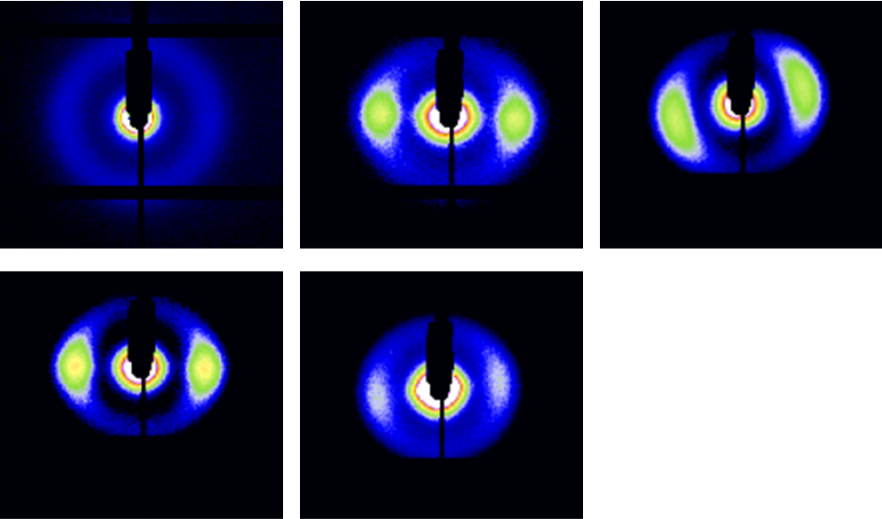
\includegraphics[width = 7.5cm, height = 4.5cm]{figures/SAXS.png}}
		\caption{The characterization of PLA/PCL blend} ~\label{fig:microstructure}
	\end{figure}
	\begin{figure}[ht]
		\centering
		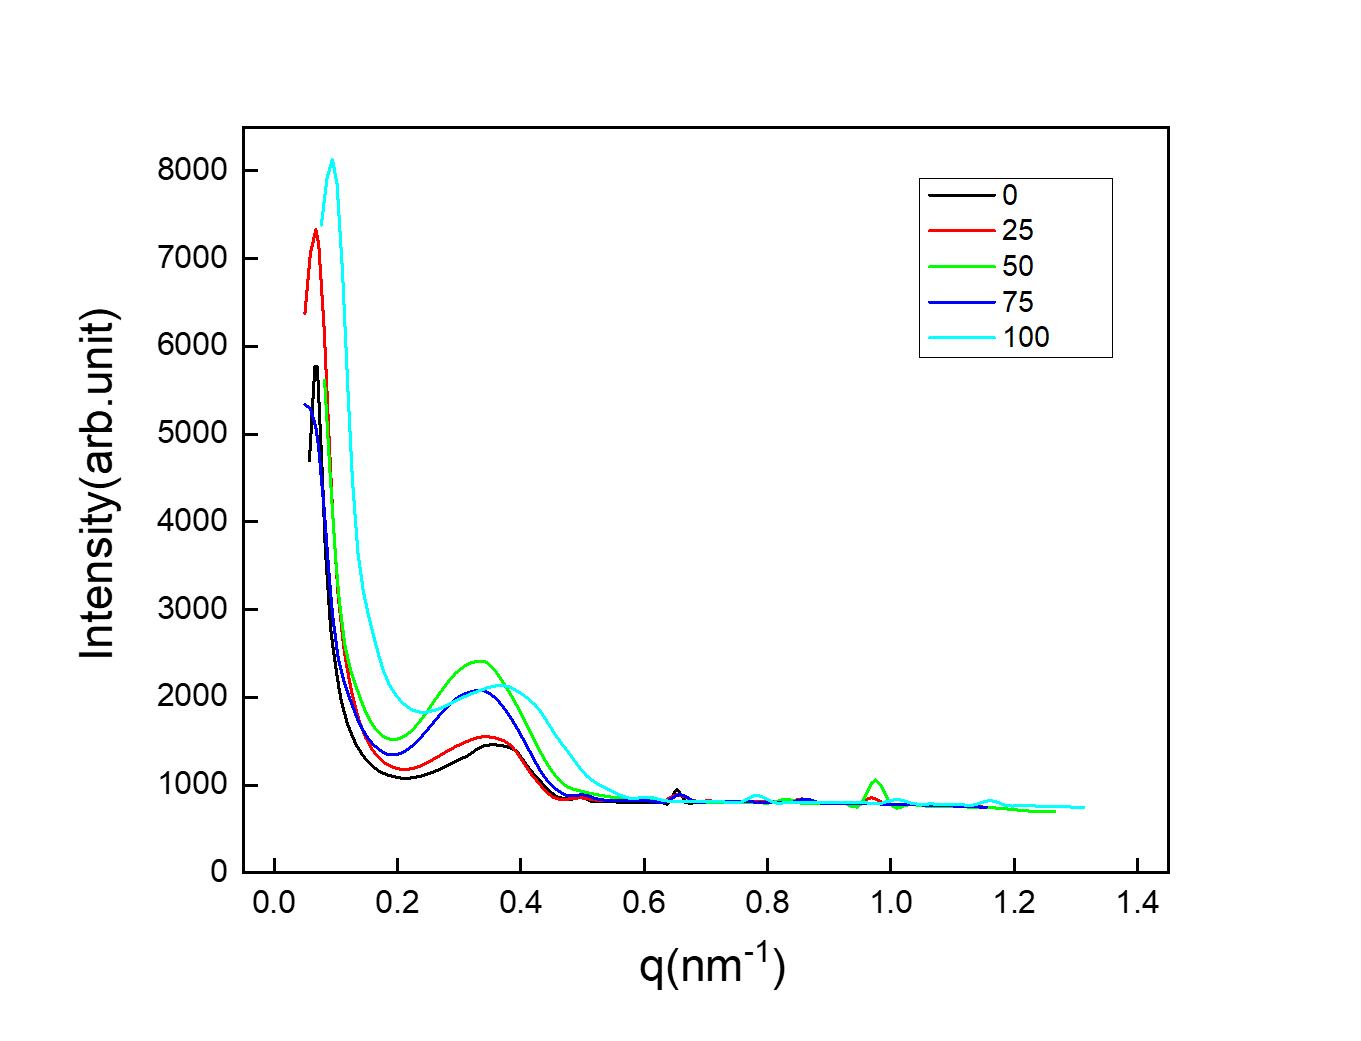
\includegraphics[scale = 0.32]{figures/IQ.png}
		\caption{The relationship plot of intensity(I) and scattering vector(Q)} ~\label{fig:IQ}
	\end{figure}
	The I-Q plot is presented in \autoref{fig:IQ}. The plot shows there is no obvious peak shift as the samples' enlongate. According to the formula $d_{\mathrm{stacking}}=\frac{2\pi}{q_{\mathrm{y,max}}}$, This result can prove that 
	no obvious lamllar width changed.


		For instance, as shown in \autoref{fig:Young} Young's modulus of the blend had a great increasement
		as the enlongation rate of the samples increased. Meanwhile, the enlongation rate at break of blends decreased slightly as the Young's modulus increased.

		In addition, the crystallization ability and crystal orientation degree of the matrix were also improved significantly in the blends due to the excellent heterogeneous nucleation ability of the PLA microfibrils.\cite{RN98}
		The results of DSC and POM showed that PCL spherulite, fan-shaped lamellae and a transcrystalline layer formed respectively under the induction effects of the PLA dispersed phases with different morphologies. In the blends, the transcrystalline layers of the PCL crystals showed a smaller average size, more crystals and stronger interface adhesion. 
		

		In conclusion, a physical treatment process to PLA/PCL blend has been carried out.
		Macroscale physical properties and microscale structure evolvement have been tested by several methods. 
		This experiment has is significant for improving the blends' dynamic properties.
	\begin{figure}[h]
		\centering
		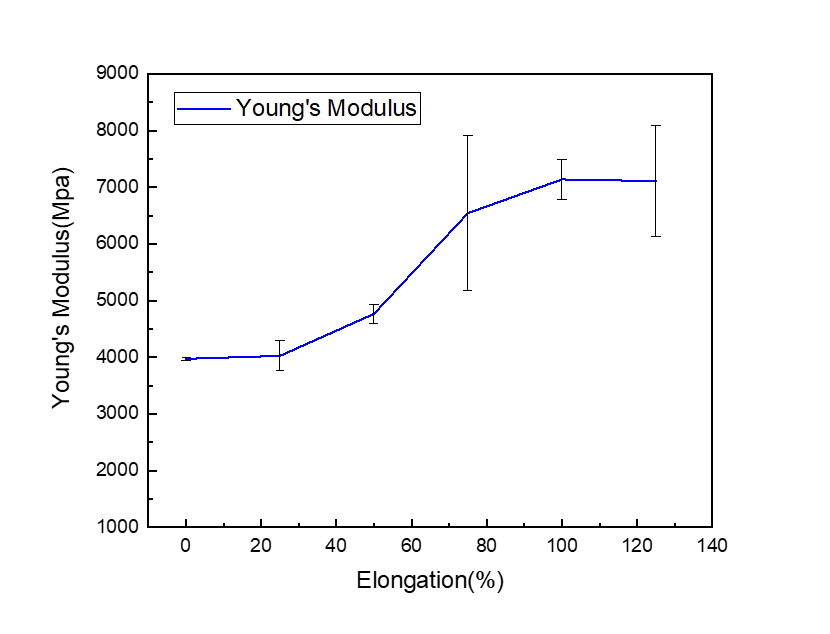
\includegraphics[scale = 0.5]{figures/Young.png}
		\caption{Young's Modulus as a function of enlongation rate of PLA/PCL polymer blends} ~\label{fig:Young}
	\end{figure}
		
	% section discussion_and_conclusion (end)
	\clearpage
	\renewcommand{\refname}{Reference}{}
	\bibliography{ref}
	% section what_can_we_get_through_saxs_method (end)
	% section section_name (end)
\end{document}
